\chapter{Background}
\label{ch:related}

%\begin{itemize}
%\item internet app is important, and more so recently
%\item some applications are dominant in terms of traffic volume, number of flow, and indespensity.
%\end{itemize}
%
%\begin{itemize}
%\item long history of research efforts
%\item change the core
%\item moving to the edge
%\item data-driven
%\end{itemize}
%
%\begin{itemize}
%\item this chapter describe architecture and related work
%\end{itemize}

Before we embark on the solutions to improve QoE, it would be helpful
to (1) motivate the need for improving QoE by shedding
light on today's QoE problems in the wild, and (2) understand the 
fundamental trade-offs in prior approaches to QoE optimization.

%as well as prior efforts towards improving application QoE.
The first part of this chapter uses empirical measurement studies to 
show that there is a substantial fraction of sessions in both Internet 
video and Internet telephony with bad QoE  
(Section~\ref{sec:related:qoe}), and then discusses 
some salient aspects of distribution infrastructures of these
applications today (Section~\ref{sec:related:back}).
%we begin with  some background information on
%Internet video and Internet telephony (Section~\ref{sec:related:back}).

The second part of this chapter discusses two research directions, 
which are closely related to this dissertation:
optimization of Internet applications quality and network performance
(Section~\ref{sec:related:quality}) and application of data-driven 
techniques to improve networked systems (Section~\ref{sec:related:data}). 
In particular, it presents a taxonomy of prior approaches to QoE optimization, 
which emphasizes the fundamental trade-off between visibility to 
user-perceived QoE and visibility to network conditions.
%these prior efforts into perspective, and
The taxonomy also helps to crystallize the contrasts between
prior work and this dissertation (Section~\ref{subsec:overview:contrast}).

\section{How Good is QoE Today?}
\label{sec:related:qoe}

We begin with large-scale measurement studies based on QoE observed 
by real users to shed light on the how good (or bad) QoE is today for 
Internet video (Section~\ref{subsec:related:video-qoe}) and Internet telephony 
(Section~\ref{subsec:related:voip-qoe}) in the wild. 
For each application, we first introduce the QoE metrics 
and the dataset, and then present empirical session-level QoE distributions
for different quality metric.

\subsection{Video QoE}
\label{subsec:related:video-qoe}

\mypara{Video QoE metrics}
We focus on  four key video QoE metrics that are common across 
different  content providers and have been shown to be
 critical for measuring quality as well as user  engagement: 
\begin{packedenumerate}

\item \emph{Buffering ratio:}  Given a video session of 
duration $T$~seconds,  if the player spent $B$~seconds in 
buffering (i.e., waiting for the 
 buffer to replenish), the buffering ratio is defined as 
 $\frac{B}{T}$. 
 Prior work has shown that buffering ratio is a key metric
 that impacts user engagement~\cite{sigcomm11}.

\item \emph{Join time:}  This is the time taken for the video 
to start playing  from the time the user clicks on the ``play'' 
button. 
While join time may not directly impact the view time of a 
specific video,
it does have long-term effects as it reduces the likelihood 
of repeated visits~\cite{sigcomm11,akamai-imc12}.  
 

\item \emph{Average bitrate:} 
Many video players today support adaptive bitrate
selection and midstream bitrate switching to adapt to 
changing bandwidth availability. 
The average bitrate of a session is the time-weighted
average of the bitrates used in a given video session. 


\item \emph{Join failures:}   Some sessions may not even 
start playing the video; either the content is not available
 on the CDN server or the CDN is under overload or other 
unknown reasons. We mark such a session as a join failure
if no content was played during this session.

\end{packedenumerate}


\mypara{Dataset} 
Our dataset is based on client-side measurements of
video  quality from over 300 million sessions over a duration
of two weeks. The unique feature of our dataset is that it is 
collected over 379 distinct content providers spanning diverse 
genres, both live and video-on-demand content, different 
content delivery platforms, different types of  bitrate adaptation 
algorithms, and device/browser platforms. 
Though US viewers dominate the dataset ($\sim$55\%), 
there are a fair number of European ($\sim$12\%) and 
Chinese ($\sim$8\%) users in the dataset.
This is especially relevant as it provides us with a panoramic 
view   of state of  Internet video delivery today.
More details on the datasets can be found in~\cite{jiang2013shedding}.

\begin{figure*}[t]
\centering
\captionsetup[subfigure]{justification=centering,farskip=-1pt,captionskip=5pt}
\subfloat[Buffering ratio]{
   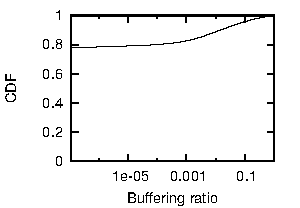
\includegraphics[width=0.32\textwidth] {figures/value_buffering.pdf}
 }
\subfloat[Bitrate]{
   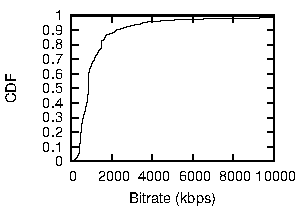
\includegraphics[width=0.32\textwidth] {figures/value_bitrate.pdf}
 }
\subfloat[Join time]{
   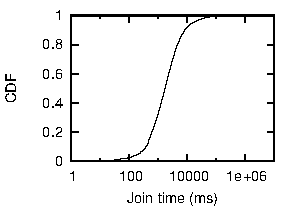
\includegraphics[width=0.32\textwidth] {figures/value_jointime.pdf}
 }
\caption{Distributions of observed video QoE metrics -- 
buffering ratio, average bitrate, and join time. 
 We see that a non-trivial number of sessions suffer quality problems. 
 For instance, more than 5\% of sessions have a buffering ratio larger
  than 10\%.  }
\label{fig:overview:qualitycdf}
\end{figure*}

\mypara{QoE distributions of different metrics}
Figure~\ref{fig:overview:qualitycdf} shows the distributions of the 
first three quality metrics over the dataset.  
(Join failures are binary events; it is not meaningful to look at a 
distribution.) 
The results reconfirm prior observations that there are a non-trivial 
number of sessions with less-than-ideal 
quality~\cite{sigcomm11,sigcomm12}. 
The key difference here is that  these past efforts only considered 
a small set of 3--4 content providers. 
In contrast,   we are considering the aggregate data from over 
300 content providers, and our results suggest that the QoE 
problems might be more pervasive than what we realized.
For instance, more than 5\% of all sessions have a join time greater 
than 10~seconds; i.e., users had to wait for 10 seconds before the 
video even started playing! Similarly, more than 5\% of sessions 
had a buffering ratio that was greater than 10\%.  
This is particularly bad as past studies show that even a 1\% 
increase in buffering ratio can lead to 3-4 minutes of lost 
viewership~\cite{sigcomm11}.  
Finally, we also see that more than 80\% of sessions observe 
an average  bitrate less than 2~Mbps; 
i.e., less than the lower end of today's ``HD'' content.   
Note that the dataset from which these observations are made
is dominated by  US-based content providers where viewers in general
have good broadband penetrations, so QoE could be even worse in 
other less developed regions.
%less than the lower end of 
%today's ``HD'' content.  





\subsection{VoIP QoE}
\label{subsec:related:voip-qoe}

\newcommand{\Call}{\ensuremath{c}\xspace}
\newcommand{\CallSet}{\ensuremath{C}\xspace}
\newcommand{\Relay}{\ensuremath{r}\xspace}
\newcommand{\RelaySet}{\ensuremath{R}\xspace}
\newcommand{\QualityFunc}{\ensuremath{Q}\xspace}
\newcommand{\HistoryCallSet}{\ensuremath{H}\xspace}
\newcommand{\Assign}{{\sf\small Assign}\xspace}
\newcommand{\Budget}{\ensuremath{B}\xspace}
\newcommand{\Predictor}{{\sf\small Pred}\xspace}
\newcommand{\BuildPredictor}{{\sf\small BuildPredictor}\xspace}
\newcommand{\GetTopK}{{\sf\small GetTopK}\xspace}
\newcommand{\Explore}{{\sf\small Explore}\xspace}
\newcommand{\Src}{\ensuremath{s}\xspace}
\newcommand{\Dst}{\ensuremath{d}\xspace}

\newcommand{\hybrid}{\textsc{Via}\xspace}
\newcommand{\Name}{Via\xspace}

\newcommand{\skype}{{Skype}\xspace}
\newcommand{\azure}{{ABC}\xspace}
\newcommand{\direct}{{default}\xspace}
\newcommand{\option}{{relaying option}\xspace}
\newcommand{\options}{{relaying options}\xspace}

\begin{figure}[t!]
\centering
\subfloat[\small{PCR vs. RTT (0.97)}]
{
        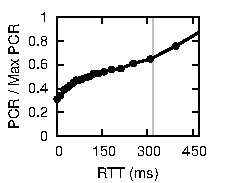
\includegraphics[width=0.3\textwidth]{figures/Via-Quality-vs-Pcr-RTT.pdf}
        \label{subfig:pcr-rtt}
}
\subfloat[\small{PCR vs. Loss (0.95)}]
{
        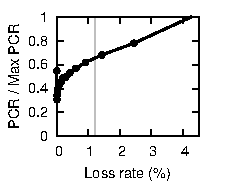
\includegraphics[width=0.3\textwidth]{figures/Via-Quality-vs-Pcr-Loss.pdf}
        \label{subfig:pcr-loss}
}
\subfloat[\small{PCR vs. Jitter (0.91)}]
{
        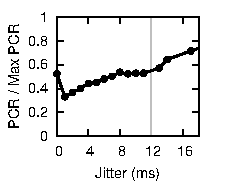
\includegraphics[width=0.3\textwidth]{figures/Via-Quality-vs-Pcr-Jitter.pdf}
        \label{subfig:pcr-jitter}
}
\caption{Network performance metrics have considerable 
impact on VoIP QoE (poor call rate or PCR); 
y-axis normalized to the maximum PCR. Vertical gray lines 
show the thresholds for poor network performance. Numbers in the
brackets show the correlation coefficients.}
\label{fig:pcr}
\end{figure}

%To quantify the call quality, we first consider an empirical approach. 
\mypara{VoIP QoE metrics}
Like video QoE metrics, VoIP QoE ideally should be based on some 
user-provided scores, but getting such information directly from users 
is not scalable.
Fortunately, for a small random fraction of calls in \skype, 
users label the call quality on a discrete $5$-point scale, 
ranging from $1$ 
(worst) to $5$ (best). This allows us to study the correlation
between these user-provided scores and network metrics that 
can be objectively measured in a scalable fashion. 
We can then use these network metrics to study the QoE 
problems across a large number of users.

Consistent with the operational practice in \skype, we deem 
the calls with a rating of $1$ or $2$ as ``poor'', and use the 
fraction of such calls, termed as the {\em Poor Call Rate (PCR)}, 
as an empirical metric of QoE. 
Figure~\ref{fig:pcr} shows the impact of the three network 
performance metrics (RTT, loss rate, jitter) on the (normalized)
user-derived PCR\footnote{Besides PCR, 
prior work also has provided analytical models to 
translate the network metrics into a measure of audio call quality, 
called the {\em Mean Opinion Score (MOS)} (e.g., \cite{cole}). 
Our study also showed that MOS is similarly correlated with
these network metrics~\cite{via}.}. 
For each network metric, we bin calls based on their 
network performance and show the PCR of the calls within 
each bin. 
For statistical significance, each bin has at least $1000$ samples. 
The figures show PCR significantly increases with all the three 
network metrics (correlation coefficients of $0.97$, $0.95$, $0.91$), 
confirming that user-perceived quality is indeed sensitive to 
network performance.
Interesting, PCR is sensitive to the {\em entire} spectrum of 
network metrics. This suggests that any improvement in RTT, 
loss or jitter is likely to improve PCR.


\mypara{Dataset}
The dataset from \skype consists of a sampled set of $430$ 
million audio calls drawn from a seven month period. 
%\camera{They are sampled from \cmvnp{the set of} calls made by \cmvnp{clients on the} \fillme platform \cmrvnp{and they are the only calls with recorded} \cmvnp{and for which} performance metrics \cmvnp{are recorded}.}
%\vnp{I wonder if the low count is because we are only considering calls for which the performance metrics are recorded. If so, we should say so.} 
The sampled set includes both calls that use the 
\direct path (e.g., BGP-derived) between the caller 
and the callee %(\cameraremove{$40\%$}\camera{$15\%$} of the calls in the set) 
as well as calls that are relayed through managed 
relay nodes distributed across datacenters in different 
locations. % (the remaining \cameraremove{$60\%$}\camera{$85\%$} of the calls). 
%\vnp{We say "randomly sampled" and then also say "sampled set is chosen" (which appears to contradictory to "random") and furthermore give the 40-60 split (which, together with "random", leaks info on how much relaying happens). I would suggest striking off "randomly".} 
Note that today such relaying is typically employed for 
connectivity (e.g., firewall or NAT traversal);
%rather than 
%for performance optimization (which is our focus here).
i.e., the only instances of relaying in our passively 
collected dataset correspond to the caller and callee being 
unable to establish a direct connection. 
Despite this bias, the dataset offers a {\em panoramic} view 
across diverse end-points from $1,905$ ASes across $126$ 
countries. 
%Table~\ref{tab:dataset} summarizes the statistics.
% \footnote{In general, it is unclear if reachability and performance are correlated.}



%In this section, we show that PCR\footnote{Besides PCR, 
%prior work also has provided analytical models to 
%translate the network metrics into a measure of audio call quality, 
%called the {\em Mean Opinion Score (MOS)} (e.g., \cite{cole}).} is
%well-correlated with network metrics. 
%Then, we identify suitable {\em thresholds} for poor call 
%performance on the network metrics of RTT, loss and jitter. 
%Since our goal is to understand the impact of network 
%performance metrics on call quality, the thresholds keep 
%our focus directly on these network metrics.
%
%\mypara{Does network performance impact user experience?}
%Figure~\ref{fig:pcr} shows the impact of the three network 
%performance metrics (RTT, loss rate, jitter) on the (normalized)
%user-derived PCR. 
%For each network metric, we bin calls based on their 
%network performance and show the PCR of the calls within 
%each bin. 
%For statistical significance, each bin has at least $1000$ samples. 
%The figures show PCR significantly increases with all the three 
%network metrics (correlation coefficients of $0.97$, $0.95$, $0.91$) 
%confirming that user-perceived quality is indeed sensitive to 
%network performance.
%Interesting, PCR is sensitive to the {\em entire} spectrum of 
%network metrics. This suggests that any improvement in RTT, 
%loss or jitter is likely to improve PCR.
%%Figure~\ref{fig:mos} shows the impact of RTT, loss rate, and jitter on MOS. %This is just a depiction of the relationship captured in the MOS equation noted above. 
%MOS (calculated using the model in \cite{cole}) also drops 
%with increase in all three metrics.

%\mypara{QoE distribution}
%We define the {\em poor network rate} (PNR) of a network 
%metric for a set of calls as the fraction of calls whose performance 
%on the metric is worse than the chosen thresholds: 
%RTT $\geq 320$ms, loss rate $\geq 1.2\%$, jitter $\geq 12$ms. 
%One of our goals is to reduce PNR of {\em each} individual metric 
% (i.e., how often each of them is poor). 


\begin{figure}[t!]
\centering
\subfloat[\small{RTT}]
{
        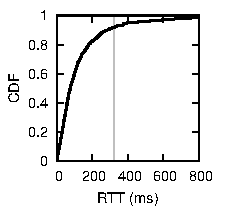
\includegraphics[width=0.28\textwidth]{figures/Via-Quality-CDF-RTT.pdf}
        \label{subfig:}
}
\subfloat[\small{Loss}]
{
        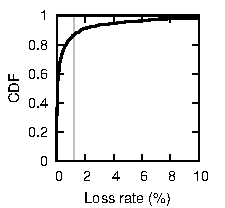
\includegraphics[width=0.28\textwidth]{figures/Via-Quality-CDF-Loss.pdf}
        \label{subfig:}
}
\subfloat[\small{Jitter}]
{
        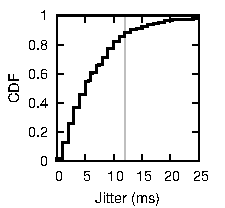
\includegraphics[width=0.28\textwidth]{figures/Via-Quality-CDF-Jitter.pdf}
        \label{subfig:}
}
\caption{Distributions of observed network performance metrics of Skype calls -- 
RTT, loss rate, jitter. Vertical grey lines show the thresholds 
for poor network performance.}
\label{fig:perf-cdf}
\end{figure}

\mypara{VoIP QoE distribution} 
Figure~\ref{fig:perf-cdf} shows the distribution of network 
performance experienced by calls  using default routes (BGP-based routes). 
The results show that a significant fraction of calls (over $15\%$) occur on paths with 
RTT over $320$ms, or loss over $1.2\%$, or jitter more than 
$12$ms, which we pick as our thresholds for 
poor performance. % These values correspond to a PCR of $0.3$ (Figure~\ref{fig:pcr}). 
%Recall from Figure~\ref{fig:perf-cdf} that these thresholds 
%correspond to the user-specified poor call rate (PCR) of $0.3$.
These thresholds are in line with literature from industry 
and standards bodies that recommend one-way end-to-end 
delay of no more than $150$ ms and a packet loss rate of 
no more than $1\%$ for good call quality~\cite{cisco-voip, itu}. 
Note that these thresholds are on the {\em average} 
values over the call's duration during which there may 
be transient spikes (e.g., loss burst) in bad performance.




\section{Today's Application Distribution Infrastructures}
\label{sec:related:back}

%This section provides some necessary background information to 
%understand the reminder of the dissertation. 

Next, we provide the necessary background on Internet video and telephony, 
focusing on the salient aspects of today's  protocols 
and distribution infrastructures.\footnote{This section is not meant for a detailed documentation of 
their end-to-end delivery systems--readers may refer to 
related work for a comprehensive 
overview of these applications' infrastructures; 
e.g.,~\cite{seufert2015survey}
for Internet videos and~\cite{baset2004analysis} for Internet telephony.} 
Specifically, we want to answer two questions:
(1) what are the tunable ``knobs'' in these applications
(Section~\ref{subsec:related:back:room} and~\ref{subsec:related:back:voip})? 
and (2) how much is the rooms for improving QoE by optimally tuning these ``knobs''
(Section~\ref{subsec:related:back:room})? 
%It is not necessary, nor practical, to describe all details. 
%Instead, I will highlight their key components relevant to this dissertation.
%For details of video streaming systems and Internet telephony
%systems, r

\subsection{Internet Video}
\label{subsec:related:back:video}

Early Internet video technologies (e.g.,  Apple QuickTime~\cite{quicktime}, Adobe Flash
RTMP~\cite{rtmp}) were  based on connection-oriented video transport protocols, 
which maintain a session  abstraction between the client and the server, 
and use (proprietary) stateful control protocols to manage the data delivery.  
The new generation of Internet video technologies such as Microsoft
SmoothStreaming~\cite{SmoothStreaming}, Apple's HLS~\cite{hls}, and Adobe's
HDS~\cite{hds}, however, are HTTP-based adaptive streaming protocols.

%\mypara{HTTP-based adaptive protocols}
In these HTTP-based protocols, each video is typically encoded at multiple 
bitrates, and is broken into 1-10 seconds chunks stored in multiple CDNs as individual files.
When a client streams a video, the player uses the HTTP protocol to fetch the chunks 
sequentially as individual web files from the server. 
Figure~\ref{fig:arch:video} gives a (simplified) depiction of the architecture
of how HTTP-based adaptive streaming protocols work in practice. 
The video chunks are stored in web servers hosted by content delivery networks
(CDNs). The video player first receives from the content provider a manifest file 
(not shown) which enumerates a list of CDNs from which the content can be 
fetched, as well as a list of available bitrates in which the content has been pre-encoded.
Then the player fetches video chunks sequentially, and 
can switch between bitrates and CDNs at the boundary of 
any two chunks. Since each chunk is fetched with an independent HTTP GET, 
there is almost no cost to switch the CDN and bitrate.
(Note that the fetches may reuse the same persistent connection 
if they are from the same CDN.)
A video is typically encoded in 3-8 bitrates, and is available from 
2-4 CDNs.


\begin{figure*}[t]
\centering
\captionsetup[subfigure]{justification=centering,farskip=-1pt,captionskip=5pt}
\subfloat[Internet video]{
   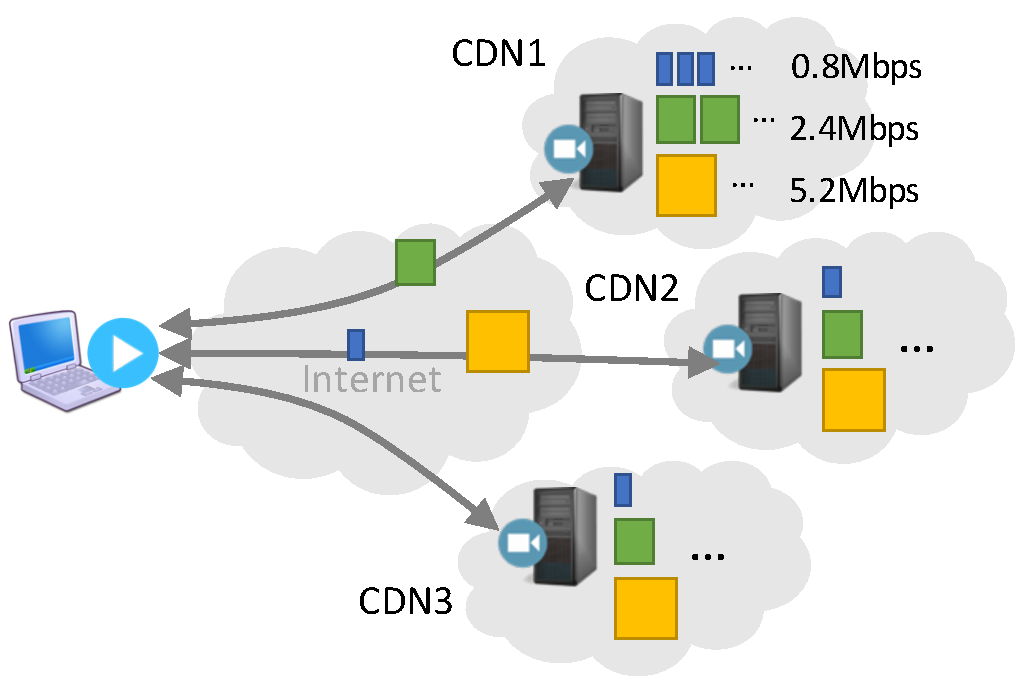
\includegraphics[width=0.5\textwidth] {figures/arch-video.pdf}
   \label{fig:arch:video}
 }
% \hspace{0.4cm}
\subfloat[Internet telephony]{
   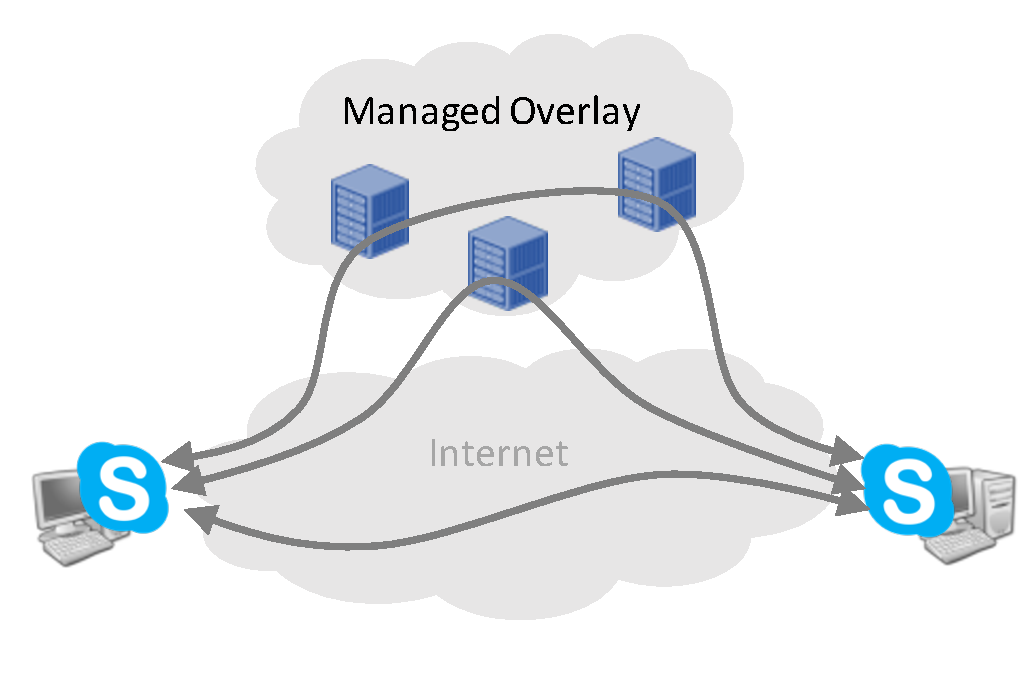
\includegraphics[width=0.5\textwidth] {figures/arch-voip.pdf}
   \label{fig:arch:voip}
 }
\caption{Today's architecture of Internet video and Internet telephony. 
Components relevant to this dissertation are highlighted; other details 
are omitted for clarity. 
The figures depict the configurations (``control knobs'')
that can be adaptively tune on a per-session/-call base in order to improve
QoE.}
\label{fig:app-arch}
\end{figure*}



%\mypara{Advantages of HTTP-based adaptive protocols} 
Compared with connection-oriented protocols, HTTP-based adaptive streaming 
protocols enjoy several advantages~\cite{festive}.
(1) The reliance on HTTP provides more ubiquitous reach and support 
as this traffic can seamlessly traverse enterprise and home
NATs and firewalls~\cite{httpwaist}.
(2)  The video servers are web servers and caches widely available from commercial
CDNs with significantly lower cost than streaming content from dedicated 
servers that support the early-generation connection-oriented video protocols.
(3) Finally, the use of HTTP as the underlying transport protocols allows 
video streaming to benefit from many techniques proposed recently to enhance
web performance and security (e.g.,~\cite{wang2014speedy}).
These practical and performance benefits have been a key driver for rapid 
growth of HTTP-based adaptive streaming protocols.



\subsection{Internet Telephony}
\label{subsec:related:back:voip}

Like Internet video, Internet telephony (or audio-video conferencing services) 
has evolved for more than a decade.
The early architecture of Internet telephony relied on peer-to-peer (P2P)
overlay systems. This key technology, called UDP hole punching, uses 
well-connected peer-to-peer users with public IP addresses 
as {\em supernodes} to enable connections between clients 
who did not have public IP addresses or were behind firewall. 
This technology led to the early success and a dramatic growth of VoIP 
services.

%\mypara{Managed overlays}
Over the past decade, VoIP services such as Skype and Google Hangouts, 
have been evolving from the traditional P2P-based overlay towards 
using {\em managed overlays} which leverage well-connected and well-provisioned 
cloud servers. 
A case in point is Skype, which started off with a peer-to-peer approach to NAT 
and firewall traversal~\cite{Skype-GI08}. 
In the recent years, Skype has adopted managed 
overlay~\cite{VideoTelephony-IMC12}, with some supernodes hosted in the 
cloud~\cite{Skype-Zdnet13}. 
It has been reported that Google Hangouts uses relays in the cloud for all 
calls, and moreover also has streams traverse the cloud backbone from one 
relay to another~\cite{VideoTelephony-IMC12}. 
Figure~\ref{fig:arch:voip} depicts a (simplified) architecture of how 
Internet telephony work over an managed overlay network.
Each call can take either the default path through the public Internet or
a {\em relayed path} that routes the traffic through
one or more relay nodes in the data centers. Relayed paths could include
a single relay to ``bounce off'' traffic or a pair of relays
to enable traffic to ``transit through'' the private backbone of
the managed overlay network.

%\mypara{Advantages of managed overlays}
While both generations of Internet telephony technologies are based on
the same technology of UDP hole punching for NAT and firewall traversal, 
the managed overlay approach enjoys several practical benefits.
(1) Global-scale managed overlays use the cloud infrastructure
which already exists and need not be built up from scratch, while 
P2P overlays involved building up overlay networks from
scratch, which limited their scale.
%, both in terms of physical infrastructure and network
%probing, which limited their scale.
(2) Supernodes in managed overlays are cloud servers
that have high available bandwidth and low latency to edge clients, 
while in P2P overlays, supernodes were regular clients, 
and they sometimes became performance 
bottlenecks due to their limited last-mile bandwidth or computational capacity.
(3) In managed overlays, communications between supernodes are
through well-provisioned private backbone networks, while in P2P overlays, all 
communications must compete bandwidth resources of public networks with
other traffic.


\subsection{Room for Improving QoE}
\label{subsec:related:back:room}

While Internet video and Internet telephony services have been 
evolving towards protocols that have less tunable knobs
(e.g., the HTTP-based streaming protocol cannot 
change bitrate arbitrarily as in traditional protocols, and 
managed overlays provide less overlay choices than 
P2P-based ones)  for practical considerations, 
these protocols still offer enough flexibility and recent research has
shown a substantial room for improving QoE by optimally selecting 
the best configuration for each application session.
%necessarily diminish the room for 
%improving QoE.
%Prior research has shown that these protocols still provide a rich set of control 
%interfaces, and there is a substantial room for improving
%QoE by selecting the right configuration for each
%session.

\begin{itemize}

\item{\em Internet video:} 
Prior research has shown that video QoE can be significantly improved
by better CDN and bitrate configuration for
each video session.
For instance, Figure~\ref{fig:back-cross-cdn} shows that there is 
significant spatial diversity and temporal dynamics of CDN 
performance~\cite{sigcomm12}.
Note that most video players today start with a statically configured 
CDN or a random CDN. This suggests a 
great opportunity of cross-CDN optimization, e.g.,
video buffering ratio can be significantly reduced by dynamically
picking the best CDN for each location and at any point of time.

\item{\em Internet telephony:}
Similarly, it has also been shown that the number of Skype 
calls whose QoE is negatively affected by network performance
can be reduced by over 50\% by judiciously selecting supernodes
to form a relay path for each Skype call~\cite{via}.
(We will elaborate on this in Section~\ref{sec:via:potential}.)


\end{itemize}

\begin{figure*}[t]
\centering
\captionsetup[subfigure]{justification=centering,farskip=-1pt,captionskip=5pt}
\subfloat[Spatial diversity]{
   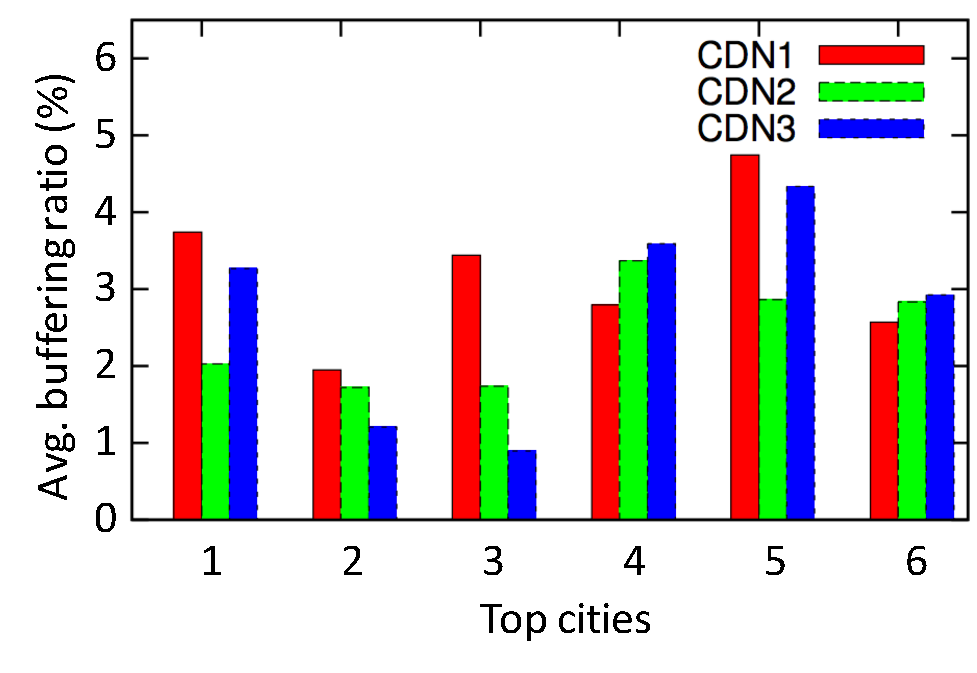
\includegraphics[width=0.4\textwidth] {figures/back-cross-cdn-spatial.pdf}
   \label{fig:back-cross-cdn-spatial}
 }
% \hspace{0.4cm}
\subfloat[Temporal dynamics]{
   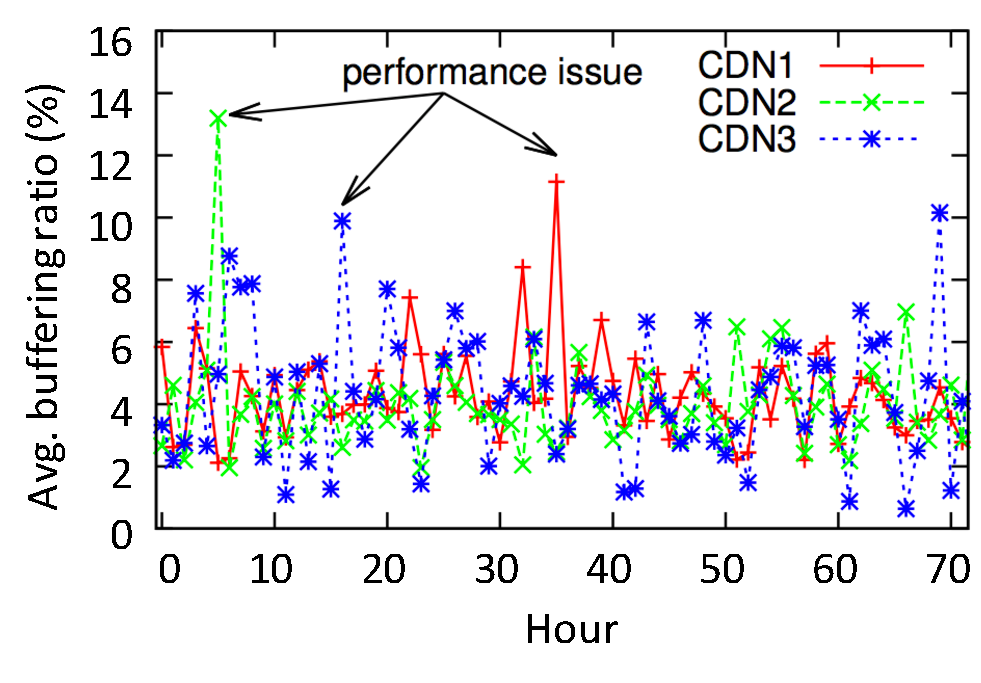
\includegraphics[width=0.4\textwidth] {figures/back-cross-cdn-temporal.pdf}
   \label{fig:back-cross-cdn-temporal}
 }
\caption{Spatial diversity and temporal dynamics of CDN 
performance~\cite{sigcomm12}. 
The figures suggest the opportunity of cross-CDN optimization:
video buffering ratio can be significantly reduced by dynamically
picking the best CDN for each location and at any point of time.}
\label{fig:back-cross-cdn}
\end{figure*}


These measurement results suggest that application QoE is 
sensitive to these configurations, and by customizing for 
each application session with the optimal parameters, 
we can substantially improve QoE over default or static 
configurations which are commonly found in today's 
implementations.


\section{Prior Work on Quality Optimization}
\label{sec:related:quality}

The evolution of the Internet has been driven largely by the need for better 
quality of a variety of applications.
%While Internet applications have always been one of the driving 
%forces behind the evolution of the Internet, 
Around early 2000s, many application providers of video streaming, 
VoIP, and web services started discovering monetization strategies, allowing 
them to scale with reduced costs. 
Since this inflection point, Internet applications have been 
growing and proliferating at an unprecedented pace.
%Especially, over the past decade, we have witnessed a drastic growth and 
%proliferation of Internet applications. 
%The inflection point occurred around early 2000s, when many application 
%providers started discovering monetization strategies for web services, 
%Internet videos, Internet telephony, and etc, allowing them 
%to scale with reduced costs.
%Today, these applications dominate the Internet traffic 
%(video traffic was 70\% of all consumer Internet traffic in 
%2015~\cite{cisco-forecast-2015}) and 
%have become indispensable for daily life
%(Skype users spend over 2 billion minutes 
%talking to each other every day~\cite{skype-2-billion-minutes}).
Not surprisingly, given the importance of Internet applications, understanding 
and improving their quality have a long history of intense research.
%Take video streaming as an example. 
%Early work in 1990s focused on providing QoS in the network, 
%and then focuses have shifted in early 2000s towards more edge-based
%and overlay-based solutions. In recent years, there is a trend to
%revisit the core-network approach enabled the emergence of 
%software-defined networks.
This section introduces a taxonomy of these prior efforts that emphasizes on 
on their inherent trade-offs.
%In Chapter~\ref{ch:overview}, we will use the taxonomy to emphasize the 
%contrast between this dissertation and prior approaches.

Before introducing the taxonomy, I would like to clarify that we use
the term ``Internet quality'' to include both quality of service (QoS) and 
quality of experience (QoE).
While QoS is different to QoE, it is closely relevant to this dissertation 
for two reasons.
First, QoS has a strong (albeit non-linear) correlation with QoE.
For instance, video buffering highly depends on packet loss, and 
VoIP call experience is very sensitive to network latency.
Second, though ultimately we care about QoE, 
much influential work has focused on providing 
QoS in the IP and transport layers.
Readers may refer to, for example~\cite{chen2015qos}, for more 
discussions on the relationship between QoS and QoE.
%can be found towards the end of this section.

\mypara{Taxonomy} 
The prior approaches to quality optimization can be categorized
based on their answers to a key architectural question: {\em where should the
functionality of quality optimization be implemented?}
There are two dimensions in the answers to the questions:
\begin{itemize}

\item {\em Where in the network?} 
There are two natural options: 
{\em endpoint-based} solutions which rely only on endpoints (e.g., clients, 
servers, caches), and 
{\em in-network} solutions which require assists from in-network devices 
(e.g., switches, routers).
To avoid any ambiguity, solutions that involve both endpoints and in-network 
devices (e.g., router-assist congestion control) fall into in-network solutions
under such dichotomy,
because they share similar advantages and disadvantages with other 
in-network solutions.
Note that although early in-network solutions only operate in or below the IP layer, 
this has since changed as in-network devices move up in the protocol stack to 
provide richer services (e.g., router-assist video 
streaming~\cite{sdndash}).

%There are two natural options: in-network and endpoints. 
%The difference between the two categories used to be straightforward--in-network 
%devices provide functionality below the IP layer for scalability, 
%while endpoints support transport- and application-layer functionality.
%The boundary, however, has become blurred as in-network devices
%move up in the protocol stack to provide richer services (e.g., router-assist video 
%streaming~\cite{bentaleb2016sdndash}).
%That said, we can still categorize prior approaches into:
%{\em endpoint-based} solutions which rely only on endpoints (e.g., clients, 
%servers, caches), and 
%{\em in-network} solutions which require assists from in-network devices 
%(e.g., switches, routers).
%The choice between endpoint-based solutions and in-network ones reflects
%the tradeoff between deployability and performance benefit; 
%while in-network solutions are arguably more difficult to be deployed 
%in practice than endpoint-based solutions, they could potentially achieve 
%better performance by finding better network paths and allocating bandwidth
%more efficiently, both of which are infeasible endpoint-based solutions.

%\item {\em What scope of measurement to drive quality optimization?}
%At one extreme, we have a purely decentralized approach where each 
%device (in-network or endpoint) or flow can improve quality by adapting 
%to network conditions inferred from its {\em locally observed} information.
%At the other extreme, we can imagine a logically centralized approach where
%the adaptation of each device or flow is driven by information from {\em multiple
%viewpoints}; e.g., from other clients of the same content provider.
%The tradeoff between the two extremes is that it may be intrinsically difficult 
%for the decentralized approach to accurately network conditions, while 
%the logically centralized approach poses additional complexity to the system, 
%e.g., gathering data from multiple viewpoints, which needs to be justified by
%improved quality.

\item {\em Which level in the protocol stack?}
Because our ultimate objective is to improve application-level QoE, 
it is natural that the solution should have access to the applications themselves,
i.e., at the application level.
That said, the layering nature of the protocol stack means that any improvement in 
the lower-level protocols (e.g., TCP, routing, wireless adaptation) may benefit the 
application-level quality.
%That said, in choosing the level in the protocol stack, there is a tradeoff between 
%more visibility to QoE and more controllability.
%On one hand, because our ultimate objective is to improve application-level QoE, 
%it is natural that the solution should have access to the applications themselves.
%On the other hand, lower layer solutions operate on a finer timescale 
%(e.g., per-packet) and have access to more feedback from the 
%Internet (e.g., packet loss), which is invisible to applications, which sometimes
%run in a user-space sandbox (e.g., browsers).

\end{itemize}




\begin{figure}[t!]
\centering
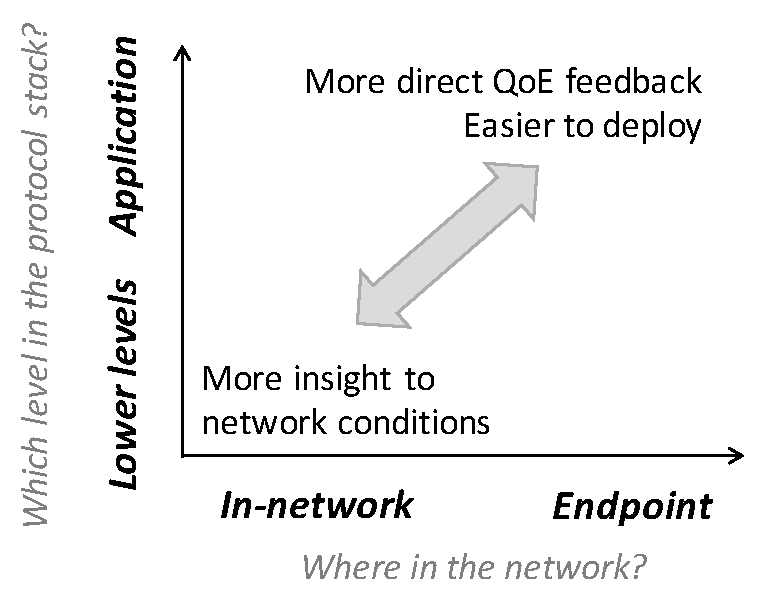
\includegraphics[width=0.5\textwidth]{figures/back-tradeoff.pdf}
%\vspace{-0.3cm}
\caption{Prior approaches can be categorized by their placement of
the functionality of quality optimization along two dimensions.
These design choices must make fundamental trade-offs between 
more visibility to QoE and more visibility to network conditions.}
\label{fig:back-tradeoff}
\end{figure}

\mypara{Design trade-offs}
The choices regarding these two dimensions involves a key architectural 
trade-off, illustrated in Figure~\ref{fig:back-tradeoff}.
\begin{itemize}

\item {\em More visibility to user-perceived QoE:} 
On one hand, optimizing quality at endpoints and the application layer has 
the advantage of more direct and accurate information on user-perceived 
QoE, which usually is available only to client-side applications.
This allows their optimization logic to be driven directly by the QoE as 
feedback. Implementing optimization functionality in endpoints at the 
application layer also carries the practical advantage of more flexibility since 
their software is upgraded more frequently than in-network devices or 
lower layer protocols.

\item {\em More visibility to network conditions:}
On the other hand, while in-network solutions in the lower layers have to rely 
on indirect metrics to infer QoE from encrypted application-level 
communications~\cite{mobicom2014-qos,
aggarwal2014prometheus,imc2012-firstbyte}, 
they enjoy the architectural advantage that they have more accurate and 
finer-grained information on the network conditions (e.g., per-packet congestion 
loss).
%which is opaque to applications typically running in a user-space sandbox 
%(e.g., browsers).
Applications running in user-space sandboxes (e.g., browsers) are often 
oblivious to changes in these low-level network conditions.

\end{itemize}



%Note that while these dimensions seem to dependent (e.g., in-network solutions
%are traditionally believed to operate only in IP layer), as we will 
%see next, they are indeed orthogonal, and there have been (or could be) 
%valid design points given each combination of answers to these questions.

Next, we use the taxonomy to put prior work in perspective.

\subsection{In-Network Solutions}
The in-network approach has long been a focus of intense research. 
In-network solutions can provide better services at multiple layers on
the protocol stack.

%\begin{itemize}
%\item QoS
%\item Router-assist TCP
%\item SDN
%\end{itemize}

\mypara{IP-layer support for QoS}
%As defined by the Internet Engineering Task Force (IETF), 
The two most prominent proposals of QoS services are
the Integrated Services (IntServ) and Differentiated Services (DiffServ). 
IntServ~\cite{intserv} uses the resource
reservation protocol (RSVP)~\cite{rsvp} to provide the
QoS by reserving resources explicitly at all routers along an end-to-end 
path, and hence all routers must keep states related to services,
leading to prohibitive scalability and complexity issues.
In contrast, the DiffServ~\cite{diffserv}
aggregates flows into pre-configured classes based on packet header 
fields, and hence is  more scalable. However, since DiffServ treats 
packets in the same class identically, it is difficult to provide QoS with
strong semantics to individual flows.
Another widely used technique is the Multiprotocol Label Switching 
(MPLS)~\cite{mpls}, which reduces 
the routing complexity and table lookups by packet labeling techniques.
Other in-network schemes also seek to provide richer services by adding
more functionality to IP layer, such as Multicast~\cite{mbone}.
With rapid growth of Internet traffic and applications, 
these early solutions have become increasingly unfit to cope
with the need for QoS with stronger semantics and 
more scalable implementation over 
an increasingly ossified infrastructure.
%The recent rapid growth of Internet traffic and applications 
%has led to the need for a solution that provide stronger QoS semantics in a 
%scalable manner, and over an increasingly ossified infrastructure.
%Hence, the basic approaches such as DiffServ and IntSev seem 
%fundamentally unfit to cope with these trends.
These trends have inspired many new in-network solutions 
over the past decade, including novel QoS service architecture (e.g., 
Core-Stateless Fair Queueing~\cite{csfq}) and clean-slate solutions (e.g.,
Active Networks~\cite{active-network}, Network OS~\cite{nox}, and 
Content-Centric Networks~\cite{ccn}).
While these efforts have enduring impact on the ensuing research,
they impose   significant deployment cost to revamp the existing ISP
infrastructure.
As a result, the Internet today still only provides best-effort
service to most applications.

\mypara{Router-assist congestion control}
While congestion control is an end-to-end functionality, many 
proposals have shown that congestion control may benefit from 
explicit router assistance, such as providing explicit or implicit 
feedback on network congestions 
(e.g., ECN~\cite{ecn},
XCP~\cite{xcp}, RCP~\cite{rcp}, VCP~\cite{vcp}),
and Active Queue management (AQM) schemes (e.g., RED~\cite{red},
AVQ~\cite{avq}, and CoDel~\cite{codel}).
In XCP and RCP, each router along an end-to-end path marks 
special bits on the packet header to help the senders determine the 
end-to-end available bandwidth. 
AQM schemes in contrast aims to prevent persistent queue buildup
in routers, by marking packets with ECN or dropping them before 
the queue is full, such as in~\cite{red}.
Similar to IP-layer support for QoS, 
these methods also add significantly complexity to in-network
devices and thus induce significant deployment cost.
Moreover, most proposals require making changes 
on all ISPs along the end-to-end paths, creating more
barriers to deployment.
A notable exception is in data centers, where 
router-assist congestion control mechanisms are widely used, 
because network devices, and end hosts are under the same 
administrative domain, and are upgraded on a regular basis.


\mypara{SDN-based approach}
SDN is a new network architecture 
to greatly simplify network management~\cite{feamster2014road}
by separating the data plane from the control plane that determines 
the routing states~\cite{OpenFlow}, thus making the data plane 
``programmable''.
The SDN-based solutions have  many open-source offerings
(e.g.,~\cite{onos,floodlightopenflow}), and offer a viable path to
the deployment of new routing 
protocols, as routing table may be updated in near real-time without
interrupting any ongoing traffic~\cite{rexford-sdn-update},
allowing routing to programmable on a per-flow basis.
Moreover, recent research on high-speed SDN-enabled routers has 
suggested that such programmability can be realized on a per-packet level 
to implement AQM schemes  in a scalable 
manner~\cite{sivaraman2016programmable,sivaraman2016packet}.
The logically centralized nature of SDN also offers an opportunity
that individual ISPs can coordinate with other ISPs
(e.g.,~\cite{schapira2010putting}) to provide end-to-end optimization
and even application QoE optimization (e.g.,~\cite{sdndash}).
%While SDN has the potential to bring ISPs into the loop of QoE optimization,
In today's federated Internet architecture, optimizing 
end-to-end quality requires multiple ISPs to coordinate, but 
even if each ISP is willing to adopt SDN paradigm for reducing management costs,
it remains unclear whether they have the incentives to coordinate
to optimize end-to-end application quality.

\subsection{Endpoint Solutions}
In contrast, the endpoint-based approach relies on endpoints to adapt to changes
in network conditions and resource availability.

\mypara{Overlay routing}
Overlay networking has been proposed as an alternative to adding functionality 
to the network core. It has been applied in a variety of contexts, such as 
virtual private networks (VPNs) and multicast~\cite{esm,ALMI-USITS01,
Multicast-Sigcomm02}. 
Of interest to us here is work focused on overlay routing with a view to improving 
routing QoS and robustness~\cite{Detour-Sigcomm99,RON-SOSP01}. 
This work showed that network performance such as 
delay, packet loss, and reliability, could be improved by using 
an overlay path that traverses well-chosen waypoints. 
Despite this promise,  overlay routing for performance gains has not seen 
much adoption in practice, for several reasons including the last-mile 
performance bottlenecks when client nodes are used as as peers, and 
the policy issues involved in turning stub networks (e.g., university campus 
networks) into de facto transit networks. 
Perhaps most importantly, these early systems operate on a relatively 
small scale (e.g., RON~\cite{RON-SOSP01} 
had tens of machines), and hence they still lack 
enough information to maintain an up-to-date view of the dynamic network 
conditions. It is also unclear whether these systems
can scale up to support today's applications running on millions of 
clients.
%involved building up overlay networks from scratch, both in terms 
%of physical infrastructure and network probing, which limited their scale.

%\mypara{CDN}


\mypara{Congestion control}
Over the past decades, TCP congestion control has received intense 
research in the literature; from the early efforts towards a 
general-purpose scheme 
(e.g.,~\cite{jacobson1988congestion,brakmo1994tcp,tcp-compound})
to later work on specializing congestion control in different operational
environments (e.g., data center~\cite{alizadeh2010data},
high bandwidth-delay product networks~\cite{cubic}, and satellite 
connections~\cite{tcp-hybla})
and to the latest efforts towards a unifying scheme by using 
machine-generated code~\cite{remy} and modeling networks 
as a blackbox~\cite{pcc}.
Current congestion control schemes suffer from a key
limitation that they only {\em react} based on the locally observed
information; e.g., without assistance of routers, they will only
react after congestion has caused packet loss or latency inflation.
A notably exception is congestion 
manager~\cite{balakrishnan1999integrated,spand},
which aggregates information of multiple TCP connections to 
predict network performance for a new connection, but these
schemes involve changing the kernel or setting up management 
server, and thus did not see wide adoption.
Moreover, state-of-the-art congestion control schemes may 
mismatch with the goal of applications~\cite{usenix12_ghobadi},
and even cause bad interaction with control loops in 
the application layer~\cite{confused,festive}, indicating that
application-layer adaptation might be in a better position to meet
the need of applications.

\mypara{Application-level adaptation}
To cope with the dynamic network conditions, 
most applications run custom client-side adaptation logics in
the application layer, rather than relying on transport-level or 
in-network solutions for two reasons:
(1) clients is in the best position to detect and respond to 
QoE problems; and 
(2) recent work suggests the need for cross-CDN 
optimizations~\cite{sigcomm12} and 
flexible web object scheduling~\cite{butkiewicz2015klotski},
which implies the need for keeping minimal state in the
network or servers.
In video streaming, most commercial products 
today perform proprietary client-side bitrate adaptation 
(e.g.,~\cite{SmoothStreaming,akamaihd,hls,netflix}) 
over HTTP-based adaptive streaming 
protocol~\cite{dash}.
Many studies have identified problems in existing
client-adaptation algorithms 
(e.g.,~\cite{mmsys2011cisco,de2010experimental}),
bad interactions with TCP control loops
(e.g.,~\cite{confused,usenix12_ghobadi}),
and techniques to improve bitrate adaptation 
(e.g.,~\cite{nossdav12_akhshabi,festive,panda}). 
Other efforts have demonstrated inefficiencies in existing 
CDN and server selection
strategies~\cite{youtubecdn,youtube-infra,sigcomm12,sigcomm12cdnmulti}.
%Many studies have shown the limitations of these 
%solutions~\cite{confused,mmsys2011cisco} and 
%proposed endpoint solutions to fix them~\cite{festive,panda}.
In Internet telephony, there has been work to improve 
client-side rate adaptation through multi-path wireless~\cite{diversifi},
network performance profiling~\cite{sprout,de2008skype}, and 
better supernode selection~\cite{baset2004analysis,Skype-GI08}).
A shared feature of these schemes is that the adaptation is driven by
local information observed by a single application session.
A notably exception is SPAND~\cite{spand}, which proposed to improve 
endpoint adaptation by sharing passive measurement from multiple 
endpoints  at the application layer.
This dissertation is in part inspired by SPAND and revisits
its ideas in the light of the advances in large-scale data analytics
and pervasive client-side instrumentations in today's Internet 
applications.


\mypara{Network performance prediction}
The key issue of endpoint adaptation is that it can only rely 
on limited, locally observed information to {\em react} to
changes in network conditions.
To overcome this limitation, many studies have attempted to 
predicting network performance, such as latency and
available bandwidth, by exploiting
stability and stationarity of network performance
(e.g.,~\cite{hu2005measurement}), constancy of various network
metrics~\cite{zhang2001constancy,balakrishnan1997analyzing}, 
and longitudinal patterns of cellular
performance (e.g.,~\cite{nikravesh2014mobile}).
%
%Moreover, measurement studies on path properties have 
%show certain stability and predictability of network performance;
%they have shown prevalence and persistence of network bottlenecks
%(e.g.,~\cite{hu2005measurement}), constancy of various network
%metrics~\cite{zhang2001constancy,balakrishnan1997analyzing}, 
%and longitudinal patterns of cellular
%performance (e.g.,~\cite{nikravesh2014mobile}).
%Inspired by these measurement studies, 
Researchers have explored three approaches to network performance prediction:
(1) to use  packet-level probes to
estimate end-to-end performance 
(e.g.,~\cite{prasad2003bandwidth,
hu2004locating, strauss2003measurement, jain2003end}),
(2) to build an ``Internet performance map''
based on active probes from a selective set of 
``vantage points'' (e.g.,~\cite{iplaneosdi, spand,ramasubramanian2009treeness,
dabek2004vivaldi}), and 
(3) to leverage the
history of the  same client-server pair 
(e.g.,~\cite{vazhkudai2001predicting,
jain2005end, swany2002multivariate,
mirza2007machine, he2005predictability}).
While this work has shown substantial benefit of accurate performance
predictions, it has not seen wide adoption for practical 
reasons: the packet-level probing requires 
per-packet information which is invisible to applications,
the Internet-map approach needs a dedicated 
monitoring infrastructure, and the history-based approach requires
enough history be accumulated before performance prediction is 
feasible, but many application sessions, such as web, 
consist of a few short-lived flows sent from different servers.



%Prior measurement studies on path properties have shown
%prevalence and persistence of network bottlenecks
%(e.g.,~\cite{hu2005measurement}), constancy of various network
%metrics~\cite{zhang2001constancy}, longitudinal patterns of cellular
%performance (e.g.,~\cite{nikravesh2014mobile}), and spatial similarity of
%network performance (e.g.,~\cite{balakrishnan1997analyzing}),
%which suggest that throughput can be predicted with reasonable 
%accuracy.



% This includes the work on  identifying
%problems \sh{existing} in client-adaptation algorithms
%(e.g.,~\cite{mmsys2011cisco}), interactions with TCP control loops
%(e.g.,~\cite{usenix12_ghobadi,nossdav12_esteban}), and techniques to improve 
%bitrate adaptation (e.g.,~\cite{nossdav12_akhshabi,festive}).  Other efforts
%have demonstrated inefficiencies in CDN and server selection
%strategies~\cite{youtubecdn,youtube-infra}.  Recent work has suggested
%cross-CDN optimizations to improve video
%quality~\cite{sigcomm12,sigcomm12cdnmulti}.


%\begin{itemize}
%\item Overlay routing
%\item CDN
%\item TCP
%\item DASH
%\end{itemize}



\subsection{Other Related Work}

Finally, we discuss other directions closely related to this dissertation.

%\begin{itemize}
%\item  QoE vs. QoS
%\item Quality measurement
%\item video related research
%\end{itemize}

\mypara{QoE metrics}
A key aspect in  video  and VoIP delivery is the need to
optimize user-perceived  QoE. While there is evidence that
video viewers are sensitive to frequent bitrate switches 
(e.g.,~\cite{user-adaptive}), sudden
changes in bitrate (e.g.,~\cite{videoqoe}), and  buffering (e.g.,
\cite{sigcomm11}), it is somewhat surprisingly challenging 
to design a good QoE metric (e.g.,
\cite{qscore}), and this is still an active area of research.
While recent work also suggests ISPs are inferring  user 
experience from network-layer measurements and QoS metrics 
(e.g.,~\cite{mobicom2014-qos,sigmetrics2014-correlation,
aggarwal2014prometheus,
imc2012-firstbyte,sigcomm2010-mercury}), we argue that 
application providers are in a better position than these 
infrastructure providers to measure and adapt to QoE.
The goal of this dissertation is not to offer new QoE models, 
but to improve  the metrics that are known to have high impact 
on user experience.

\mypara{Video measurements}
There are many recent measurement studies on
understanding video content popularity and access patterns
(e.g.,~\cite{youtube-imc07}\cite{plissonneau2012longitudinal}), 
flash crowds during highly popular events (e.g.,~\cite{beijing-imc09}), 
and their implications for CDN and caching designs.  
While these efforts help motive the techniques proposed in 
this dissertation, our goal again is to understand the structure of 
quality problems and further develop solutions to actually improve
QoE.

\vspace{0.5cm}
While both in-network solutions and endpoint solutions have 
to compromise on either visibility to QoE or visibility to network conditions,
the solutions proposed in this dissertation 
strikes a better balance by taking advantage of the access of millions of 
endpoints with a data-driven approach.
%enabling an endpoint-based data-driven approach.


\section{Prior Work on Data-Driven Optimization in Networking}
\label{sec:related:data}

Another direction closely related to this 
dissertation is the application of the data-driven paradigm to improving 
networked systems. 
We introduce a taxonomy of how networked systems can benefit from the 
data-driven paradigm.
We also use a concrete case study to show how data-driven ideas can
be applied to improve TCP congestion control in different ways. 

While most systems already use data-driven techniques 
(e.g., TCP congestion control schemes react against congestion 
signals such as packet loss and round-trip time),
we argue that they could be substantially
improved by borrowing systematic frameworks from data science
literature and further exploring more data-driven opportunities by
leveraging more available data.
In particular, we observe two aspects of network systems along 
which the data-driven paradigm can help:
{\em better setting of parameters} within the existing adaptation logic,
and {\em better run-time decision making logic} to replace the existing one.

Since the way in which networking problems benefit from data-driven 
techniques bears much resemblance to 
other systems areas, 
this section will focus on networking problem, but also draw 
related work from a broad set of systems areas.

\subsection{Type I: Better Settings of Parameters}
\label{subsec:related:data:type1}

The conventional wisdom has been that in most of network protocols, 
the adaptation should use {\em hand-picked} parameters, (e.g., TCP parameters 
such as initial congestion window size and AIMD parameters).
Recent research, however, has shown that performance
can be improved by {\em automatically} tweaking these parameters 
to achieve better performance in different operating conditions
(e.g., better parameters of TCP congestion control~\cite{remy,googleinitwindow}, 
AQM logic~\cite{shah2016sam,lin2015kemy}), configurations of routing algorithms 
(e.g.,~\cite{sharma2017machine}, and workload modeling in wireless 
networks~\cite{alsheikh2014machine}).
Recent research has also shown similar data-driven opportunities 
in other areas including CPU cache replacement policy~\cite{calvinlin-cache},
database consistency management~\cite{aaron-cidr}, and 
rational database system management~\cite{andypavlo-rbsm}.
While these efforts are in entirely different areas, they have largely 
exploited the same inefficacy in traditional
control logic that the parameters are statically configured 
based on assumptions that are ill-matched with the dynamic workload 
in runtime.  
Such problem can be fixed by dynamically training
these parameters with recent measurements
(e.g.,~\cite{calvinlin-cache}) or synthetically simulated data (e.g.,~\cite{remy}).
The problem of learning the best configurations
for a complex system is conceptually similar to the 
hyper-parameter selection problem in machine learning~\cite{ml101}.

\noindent\underline{\smash{Case study: Tunning congestion control parameters:}}
We use TCP congestion control as a case study to show
how a protocol can be improved by tuning the key parameters.
%In Remy~\cite{remy}, if we want to optimize for a given 
%performance metric (e.g., flow completion time) under 
%some given network characteristics 
%(e.g., mean round-trip time and packet loss rate), Remy 
%can train key congestion control parameters such as 
%AIMD parameters and the timeout threshold using offline
%simulation against traffic synthetically generated based on
%the given network characteristics.
Prior work on Remy~\cite{remy} showed that a machine-designed 
TCP that uses offline simulation driven by prior  knowledge of the 
network context (e.g., topology, degree of multiplexing) can learn 
the best values of some key constants and achieve significant 
performance improvement over today's manually picked values; 
e.g., a simulated 15 Mbps fixed-rate link with eight senders 
contending and an RTT of 150 ms, Remy-generated control logic achieves 
40+\% throughput speed up and 20+\% delay reduction over many 
specially engineered TCP variants.


%\begin{itemize}
%\item TCP
%\item Cache replacement
%\item database configurations
%\end{itemize}

\subsection{Type II: Better Run-Time Decisions}
\label{subsec:related:data:type2}

While finding better parameters of the existing control logics
can improve performance, it is arguably incomplete, since it still uses 
handcrafted control logics based on analytical model that models the 
relationship between the feedback signals (e.g., RTT) with internal states of the 
underlying system (e.g., router queue occupancy). 
While this approach served us well for decades, it is fundamentally inefficient 
to characterize today's application delivery systems, which have grown too 
complex to model analytically. Rather than merely tuning the parameters for 
the existing control logic, recent research has made a case for a 
more direct approach in which the logic models the network as a 
blackbox and use measurement data to drive the decision making.
In other word, rather than inferring the underlying network states and finding
best decisions analytically, it builds a model that directly associate quality
feedback with decisions (configurations).
Research has shown that this more direct data-driven 
approach can improve the performance of routing~\cite{schapira2010putting},
TCP throughput~\cite{pcc}, server selection in web 
performance~\cite{footprint}, as well as bitrate adaptation in 
video streaming~\cite{neural-streaming}.
Besides networking problems, this approach also found its
application in improving resource scheduling in 
cloud services~\cite{cherrypick}.
%The basic idea of this type of data-driven approach is
%build a blackbox model to describe the relationship between 
%action (decisions) and performance feedback, 
The techniques commonly used in these solutions are largely based on 
exploration-exploitation strategies (multi-armed techniques~\cite{mab}), or 
Bayesian optimization~\cite{bayesian-optimization}), in which feedback of 
network performance is used to explore the decision spaces.
Compared to the first type, the main advantage of the 
second type is that it could converge to a better decision
faster by making minimal assumption about the 
underlying  systems. 
A primary drawback, however, is that it has less interpretability
as the underlying system is modeled as a blackbox.


\noindent\underline{\smash{Case study: Blackbox-based congestion control:}}
Again, we use TCP congestion control as a case study to show
how a protocol can be transformed to a simpler logic driven
completely by measurement data, while making less
assumptions on the underlying network system.
PCC~\cite{pcc} attempts to simplified TCP congestion 
control algorithm by using locally observed performance 
to directly drive the setting of congestion window size. 
Specifically, it continuously maintains a model between 
observed performance (e.g., throughput and latency) 
and cwnd. This approach greatly simplifies TCP congestion
control, while at the same time, significantly 
improves TCP performance; e.g., 10$\times$ higher
throughput of TCP CUBIC on global commercial Internet.

%\begin{itemize}
%\item video streaming
%\item pcc
%\item routing
%\end{itemize}

%The boundary could be blurred

%mention KnowledgePlane

%\subsection{Discussion}
%
%There are three final remarks regarding the the various ways the 
%data-driven paradigm is applied in networking research:
%
%%\mypara{Data-driven and ML-based diagnosis} 
%First, while we focus on using data-driven technique for 
%better adaptation, many efforts have shown similar data-driven 
%opportunities in better diagnosis of complex network systems~\cite{knowledgeplane,attmanagement}.
%
%%\mypara{} 
%Second, the boundary between these two types of data-driven 
%approaches is in fact not as clear as we discussed. 
%
%Finally, while the Type II approach uses more real-time data
%to directly drive the adaptation, it only leverages the same
%data available to other prior work. In endpoint solutions,
%it would be fundamentally limited by the scale and scope 
%of the locally measurable data.


\section{Summary}

In the first part of this chapter, we have used empirical studies 
to show that QoE problems are pervasive in Internet video and Internet 
telephony. Then we have introduced related background on today's 
Internet video and Internet telephony services.

In the second part of this chapter, we have introduced a taxonomy
to highlight the inherent trade-offs in prior work to improve Internet 
application quality. %--in-network solutions and endpoint solutions.
%In particular, we have focused on the architectural trade-offs
%in their placement of the functionality of quality optimization.
In-network solutions have more direct and accurate visibility to 
network conditions, while endpoint solutions can measure metrics
more directly related to user-perceived QoE, and are  usually more deployable.
%While prior work has to compromise on at least one front,
As we will see, our solution strikes a better balance
between the visibility to user-perceived QoE and the visibility to 
network conditions through taking a more data-driven approach to 
endpoint solutions.

In the last section, we have discussed two approaches to using the
data-driven paradigm to improve network systems: improving setting
of parameters, and improving real-time decision-making logic.
While our solution follows the second type, it unleashes more 
data-driven benefit by taking advantage of more data of real-time 
measurements collected from millions of endpoints.





